% template
\section{Template matching}
We use templates with high SNR to detect events strongly resemble templates through stacking P wave cross-correlograms and S wave cross-correlograms between the template waveforms and potential event signals in the continuous records over multiple stations and components. The templates are got by short-term average(STA)/long-term average(LTA) method. The Figure \ref{fig:method} shows one example of this method.
\begin{figure}[htbp] 
\centering 
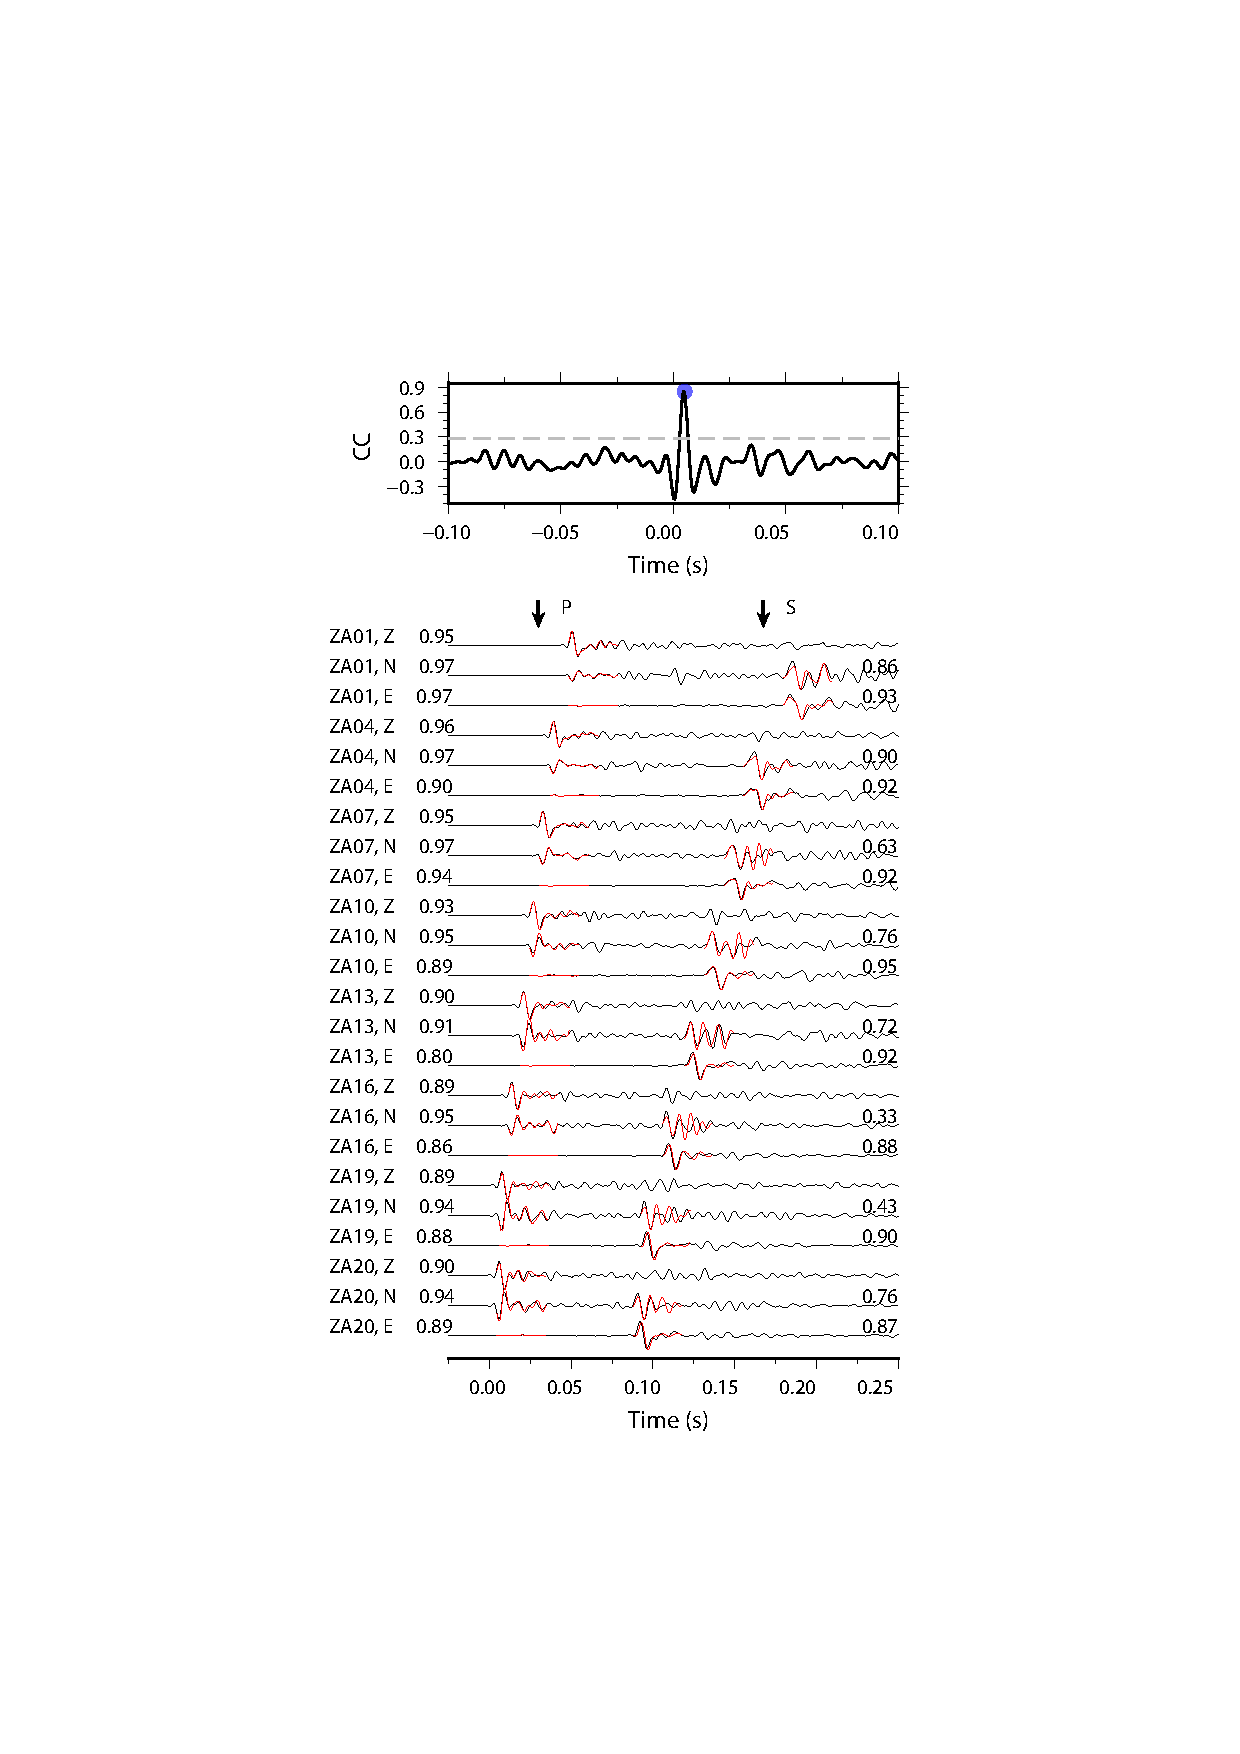
\includegraphics[trim=4cm 5cm 4cm 5cm,, clip,  width=0.7\textwidth]{Template-search} 
\caption{\label{fig:method} (a) Stacked cross-correlograms. (b) Waveform comparison between the master event (red) and the target slave event (black) for the three components of several selected receiver levels.} 
\end{figure}
In this project, we use 14 templates and detect 22 events. Among the 22 events, there are 8 events can obviously observed.

